\chapter{Third Sprint}

This chapter covers the development done during the third sprint, which is primarily about the systems analytical ability. During this chapter we will explain how we use kernel estimation to calculate the crowd conditions that were introduced during the first sprint. Afterwards we will explain the design of the analyser, which is the software module that will execute the kernel estimation of the crowd conditions. Then at the end we will discuss implementation of this module. Unlike the other sprints, we will not conclude this sprint based on a meeting with Alarm HS of SmukFest, but will instead do internal assessment of the analytical ability of the system.

%% requirements specification
\section{Requirements Specification} \label{sec:s3_requirements}
% Update intro.....


Based on the feedback received from the second Alarm HS meeting, additional requirements will be added to the requirement specification from \cref{sec:s2_reqs}. This gives the following requirement specification.

\subsection{Additional Users} \label{ss:s3_users}
% Users: festical guest, guards, medical personnel

\subsection{Additional Use Cases \label{ss:s3_uc}}
% add use cases

\subsection{Revised Requirements} \label{ss:s2_reqs}
Based on the new use cases several additional functional requirements have been identified, which must be added to the requirements previously identified in \cref{ss:s2_update_reqs}. The following requirements will be added:

\begin{enumerate}
    \item \emph{A map legend.} In order to make the crowd information overlays more intuitive, a map legend explaining the overlays must be added. This is very important for a usable system, and will be prioritised as must have.
    \item \emph{Multiple access levels.} The system must have multiple access levels, such that information and features can be targeted at the relevant users. This is important for the system, is prioritised as must have.
    \item \emph{Adding of markers at specific locations.} These markers could be used to contain information of incidents, and should be visible to all relevant users. This is prioritised as should have.
    \item \emph{A help feature.} The application should have a help feature that explains the applications functionalities. This is prioritised as should have.
    \item \emph{Send notification to other users.} It could be possible for some users with a sufficient access level to send notification to other users. This is prioritised as could have.
    \item \emph{A menu with searchable contact information.} A menu containing the contact information of the festival employees. It should be possible to search through the contacts. This is prioritised as won't have, as it is not important for the usability of the application.
    \item \emph{Reporting of incidents by festival guests.} It could be possible for festival guests to access the application, and report an incident on the map. This requirement is not in the scope of the project, and is prioritised as won't have.
\end{enumerate}

Updating the previous requirements specification from \cref{tab:s2_req} gives us the requirement specification shown in \cref{tab:s3_req}.

\begin{table}[h!]
	\centering
	\begin{tabularx}{\textwidth}{lXl}
		\toprule
		\textbf{ID} & \textbf{Requirement} & \textbf{Priority} \\
		\midrule 
		\rowcolor[HTML]{EFEFEF} 
		S1-FR1 & A detailed map of the area & Must have \\
		S2-FR1 & A map overlay that intuitively visualises crowd density & Must have \\
		\rowcolor[HTML]{EFEFEF} 
		S2-FR2 & A map overlay that intuitively visualises crowd velocity & Must have \\
		S2-FR3 & A map overlay that intuitively visualises crowd turbulence & Must have \\
		\rowcolor[HTML]{EFEFEF} 
		S2-FR4 & A map overlay that intuitively visualises crowd pressure & Must have \\
		S1-FR3 & A graphical user interface for desktop computers & Must have \\
		\rowcolor[HTML]{EFEFEF} 
		S1-FR4 & A graphical user interface for smartphones & Must have \\
		S2-FR5 & Layers of details that can be toggled on and off & Must have \\
		\rowcolor[HTML]{EFEFEF} 
		S2-FR6 & User authentication & Must have \\
		S3-FR1 & A map legend & Must have \\
		\rowcolor[HTML]{EFEFEF}
		S3-FR2 & Multiple access levels & Must have \\
		S2-FR7 & A search function & Should have \\
		\rowcolor[HTML]{EFEFEF}
		S3-FR3 & Adding of markers at specific locations & Should have \\
		S3-FR4 & A help feature & Should have \\
		\rowcolor[HTML]{EFEFEF} 
		S2-FR8 & Navigation assistance & Could have \\
		S2-FR9 & Automatic warning system & Could have \\
		\rowcolor[HTML]{EFEFEF} 
		S2-FR10 & A visualisation of available personnel & Could have \\
		S3-FR5 & Send notification to other users & Could have \\
		\rowcolor[HTML]{EFEFEF}
		S2-FR11 & Projection onto camera images & Won't have \\
		S3-FR6 & A menu with searchable contact information & Won't have \\
		\rowcolor[HTML]{EFEFEF}
		S3-FR7 & Reporting of incidents by festival guests & Won't have \\
		\bottomrule
	\end{tabularx}
	\caption{Functional requirements for the third sprint.}
	\label{tab:s3_req}
\end{table}

No non-functional requirements are added in this sprint, so the non-functional requirements are still given by \cref{tab:s2_nreqs}.

% Or is this a non-functional requirement?? TBD
\textbf{Should have}
\begin{enumerate}[resume]
    
    \item \textbf{[Added]} All data displayed to the user could also be stored for later retrieval, allowing for analysis of a problematic situation, which could improve the ability to handle similar future situations.
    
\end{enumerate}


%% kernel theory
\section{Kernel Density Estimation}

\kanote{introduktion til kernel density - HUSK at skriv motivation om hvorfor vi skal vide hvordan man udregner det her, samt hvordan det binder sammen med tidligere afsnit}

This section will first explain how kernel density estimation is used to estimate the local crowd density. Afterwards, we explain how this approach can be extended to estimating velocity, turbulence, and pressure.


\subsection{Kernel Density Estimation}
\label{sub:kernelDensityEstimation}

Finding a local crowd density can be a simple task. Simply define the local area, and count the number of people inside that areas, and divide it by the size of the local area. This process could then be repeated across multiple local areas, to give us the the local densities across the entire area. These counts could then be displayed in histograms for a better overview. The problem with this approach is the definition of the local areas. Whatever way you decide to define the areas will affect the outcome of the count, which in turn will affect the histograms, giving a possibly skewed overview\kanote{jens, insert article reference here}. Since we do not want this, we need to use a different method.

%--- Jens' formulering --- %
%To calculate the local crowd density, one could place a grid over the area, count the number of people in each square and divide by the area of the square. This can be done with histograms. The problem with this method is its sensitivity to the grid, and that inaccuracies in the measured positions are not accounted for.\jenote{Complete the argumentation for why we should use kernel density estimation rather than histograms}

\kanote{mangler en overgang fra problemet med histogrammer til kernel density estimation}

There exists multiple kernel functions that can be used in the kernel density estimation. The most commonly used is the Gaussian distribution, also known as the normal distribution, given by the function in \cref{eq:1dGaussianDistribution}. The function, given the distance $d$ from an observation to the center of the kernel, returns the probability of the observation. An observation in this context, is a sample drawn from the distribution. The Gaussian distribution is commonly used as a kernel function because it arises naturally, both in theory and in experiments.

\begin{equation}
\label{eq:1dGaussianDistribution}
K(d) = \frac{1}{\sqrt{2\pi}} e^{-\frac{1}{2} d^2}
\end{equation}

The plot of the function is shown in \cref{fig:1dGaussianDistributionPlot}. Notice that the function only converges with the x axis in $-\infty$ and $\infty$. This means that if we were to use this function for calculating the local crowd density, we would have to consider every person in the data set, because the function is defined for every x value. For performance reasons, this is not preferable.

Another kernel function is the Epanechnikov kernel, given by the function in \cref{eq:1dEpanechnikovDistribution}.

\begin{equation}
\label{eq:1dEpanechnikovDistribution}
K(d) = \frac{3}{4} \left( 1-d^2 \right) \mathbbm{1}_{\{\left| d \right| \leq 1\}}
\end{equation}

Here $\mathbbm{1}_{\{|d| \leq 1\}}$ denotes the indicator function, meaning that if $|d|$ has a value less than or equal to 1, the function returns $1$, otherwise $0$. This means that any person placed outside this range in our data set can be ignored. This property can be seen in the plot of the function in \cref{fig:1dEpanechnikovDistributionPlot}, where one can also see that the function converges with the x axis at $-1$ and $1$.
\lanote{Maybe remove this graph and use the one with the area marked instead}

\begin{figure}[htbp]
\begin{subfigure}[c]{.49\linewidth}
    \centering
    \begin{tikzpicture}[scale=0.9]
    \begin{axis}[
    axis y line=center,
    axis x line=middle,
    grid=both,
    xmin=-3,xmax=3,
    ymin=-0.2,ymax=1,
    xlabel=$x$,ylabel=$y$,
    x label style={at={(axis description cs:1,0.2)},anchor=east},
    y label style={at={(axis description cs:0.5,1)},anchor=north west},
    xtick={-3,-2,-1,0,1,2,3},
    ytick={-0.2,0,0.1,0.2,0.3,0.4,0.5,0.6,0.7,0.8,0.9,1},
    height=7.5cm,
    anchor=center]
    \addplot[mark=none, thick, samples=100, smooth, domain=-1:1] {epanechnikov2d(1)};
    \addplot[mark=none, thick, samples=100, smooth, domain=1:3] {0};
    \addplot[mark=none, thick, samples=100, smooth, domain=-1:-3] {0};
    \end{axis}
    \end{tikzpicture}
    \caption{Epanechnikov distribution}
    \label{fig:1dEpanechnikovDistributionPlot}
\end{subfigure}
%
\begin{subfigure}[c]{.49\linewidth}
    \centering
    \begin{tikzpicture}[scale=0.9]
    \begin{axis}[
    axis y line=center,
    axis x line=middle,
    grid=both,
    xmin=-3,xmax=3,
    ymin=-0.2,ymax=1,
    xlabel=$x$,ylabel=$y$,
    x label style={at={(axis description cs:1,0.2)},anchor=east},
    y label style={at={(axis description cs:0.5,1)},anchor=north west},
    xtick={-3,-2,-1,0,1,2,3},
    ytick={-0.2,0,0.1,0.2,0.3,0.4,0.5,0.6,0.7,0.8,0.9,1},
    height=7.5cm,
    anchor=center]
    \addplot[mark=none, thick, samples=100, smooth] {gaussian2d(1)};
    \end{axis}
    \end{tikzpicture}
    \caption{Gaussion/normal distribution}
    \label{fig:1dGaussianDistributionPlot}
\end{subfigure}
\caption{Kernel density function plots}
\end{figure}

Choosing a kernel function is not very important as long as the chosen function has an area of 1 beneath it.\jenote{find source} The area of both functions can be seen plotted in \cref{fig:1dGaussianEpanechnikovAreaPlot}. While both Gaussian and Epanechnikov hold this property, Epanechnikov was chosen because it is not defined for every x value, making its performance advantageous. There are many other kernel functions that also apply the indicator function and has an area of 1 beneath its curve which could have been considered. However since the choice of the kernel function is of minor importance, we did not pursue other options.

\begin{figure}[htbp]
\begin{subfigure}[c]{.49\linewidth}
    \centering
    \begin{tikzpicture}[scale=0.9]
    \begin{axis}[
    axis y line=center,
    axis x line=middle,
    grid=both,
    xmin=-3,xmax=3,
    ymin=-0.2,ymax=1,
    xlabel=$x$,ylabel=$y$,
    x label style={at={(axis description cs:1,0.2)},anchor=east},
    y label style={at={(axis description cs:0.5,1)},anchor=north west},
    xtick={-3,-2,-1,0,1,2,3},
    ytick={-0.2,0,0.1,0.2,0.3,0.4,0.5,0.6,0.7,0.8,0.9,1},
    height=7.5cm,
    anchor=center]
    \addplot[mark=none, thick, samples=100, smooth, domain=-1:1] {epanechnikov2d(1)};
    \addplot[mark=none, thick, samples=100, smooth, domain=1:3] {0};
    \addplot[mark=none, thick, samples=100, smooth, domain=-1:-3] {0};
    \addplot[mark=none, thick, samples=100, smooth, fill=lightgray, fill opacity=0.5, domain=-1:1] {epanechnikov2d(1)};
    \end{axis}
    \end{tikzpicture}
    \caption{Epanechnikov distribution}
    \label{fig:1dEpanechnikovAreaPlot}
\end{subfigure}
%
\begin{subfigure}[c]{.49\linewidth}
    \centering
    \begin{tikzpicture}[scale=0.9]
    \begin{axis}[
    axis y line=center,
    axis x line=middle,
    grid=both,
    xmin=-3,xmax=3,
    ymin=-0.2,ymax=1,
    xlabel=$x$,ylabel=$y$,
    x label style={at={(axis description cs:1,0.2)},anchor=east},
    y label style={at={(axis description cs:0.5,1)},anchor=north west},
    xtick={-3,-2,-1,0,1,2,3},
    ytick={-0.2,0,0.1,0.2,0.3,0.4,0.5,0.6,0.7,0.8,0.9,1},
    height=7.5cm,
    anchor=center]
    \addplot[mark=none, thick, samples=100, smooth] {gaussian2d(1)};
    \addplot[mark=none, thick, samples=100, smooth, fill=lightgray, fill opacity=0.5, restrict y to domain=0:1] {gaussian2d(1)};
    \end{axis}
    \end{tikzpicture}
    \caption{Gaussian/normal distribution}
    \label{fig:1dGaussianAreaPlot}
\end{subfigure}
\caption{The area beneath both Epanechnikov and the Gaussian distribution}
\label{fig:1dGaussianEpanechnikovAreaPlot}
\end{figure}

A kernel density estimation is performed for a specific point, and can be calculated as either absolute, relative, or probabilistic density. The absolute density is the amount of people per local crowd density point. This means that the densities for all points have to sum up to the total amount of people.

The relative densities are the absolute densities divided by the area that each point covers, for instance people per square meter. Since we want to be able to compare the values calculated for the crowd factors with certain limits, this is the type of kernel density we want to calculate.

The last kernel density type is probabilistic. This is the absolute densities divided by the total amount of people, meaning that the total sum of probabilistic local crowd densities has to be 1.

Kernel functions have an area of 1 beneath them since they denote the probability of finding an observation at certain distances from them. In essence this means that all observations exist in the distribution of the function. In our case, this denotes how much an observed person weighs for the density of the point. The problem is that observations can exist further away than a distance of 1. We assume that all distances are in SI unit meters. We want a way to raise or lower the distance of observations that should be considered in the estimation, in order to include all observations of importance, but still have the kernel density functions have an area of 1. This is done using a bandwidth variable. The Epanechnikov function with the bandwidth can be seen in \cref{eq:1dEpanechnikovDistributionWithH} and the plot of the function is shown in \cref{fig:1dEpanechnikovDistributionWithHPlot} with the area underneath. The area of this function is still 1 and therefore holds the property of a kernel density function.

\begin{equation}
\label{eq:1dEpanechnikovDistributionWithH}
K(d) = \frac{3}{4 h} \left( 1-\left(\frac{d}{h}\right)^2 \right) \mathbbm{1}_{\{|u| \leq 1\}}
\end{equation}

Here $d$ is the distance from the center of the kernel function to the observation, and $h$ is the bandwidth.

\begin{figure}
\centering
\begin{tikzpicture}[baseline]
\begin{axis}[
axis y line=center,
axis x line=middle,
grid=both,
xmin=-6,xmax=6,
ymin=-0.2,ymax=1,
xlabel=$x$,ylabel=$y$,
x label style={at={(axis description cs:1,0.2)},anchor=east},
y label style={at={(axis description cs:0.5,1)},anchor=north west},
xtick={-5,...,5},
ytick={-0.2,-0.1,0,0.1,0.2,0.3,0.4,0.5,0.6,0.7,0.8,0.9,1},
width=10cm,
height=7.5cm,
anchor=center]
\addplot[mark=none, thick, samples=100, smooth, domain=-6:-5] {0};
\addplot[mark=none, thick, samples=100, smooth, domain=5:6] {0};
\addplot[mark=none, thick, samples=100, smooth, fill=lightgray, fill opacity=0.5, domain=-5:5] {epanechnikov2d(5)};
\end{axis}
\end{tikzpicture}
\caption{The area beneath the Epanechnikov function with bandwidth 5}
\label{fig:1dEpanechnikovDistributionWithHPlot}
\end{figure}

Currently we have only been looking at the distribution over one dimension. In our domain we get observations from a plane, in two dimensions. We can extend the kernel function to work on a two dimensional area by calculating the distance from the kernel function center point to the desired point in two dimensions. In 2 dimensions, the distance would be the same as a radius in a circle. This can be seen plotted in \cref{fig:3dEpanechnikov}.

\begin{figure}[htbp]
\centering
    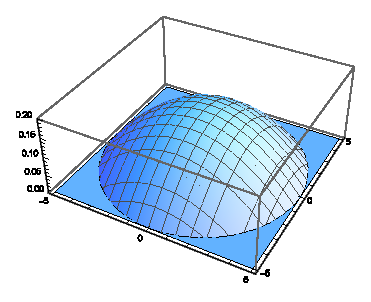
\includegraphics[width=0.5\textwidth]{3dEpanechnikov.eps}
    \caption{Epanechnikov over an area shown in 3 dimensions.}
    \label{fig:3dEpanechnikov}
\end{figure}

\Cref{fig:3dEpanechnikov} represents the distribution over a 2 dimensional space, where the third dimension represents how much the 2 dimensional points weights.

As explained earlier, the function is currently on a probability form, and not on the desired relative density form. In order to modify it, we first transform it to an absolute form. People closer to a point will weigh more than people further away from the point. We assume that every person contributes the same density, so the mean value of the function should be 1. In order to \enquote{raise} the function so the mean value is 1, we can divide by the volume beneath the plane and multiply with the desired volume. The desired volume is that of which the kernel function has a mean value of 1. We start by calculating the current volume beneath the plane. This can be done through a triple integration on the function using a circular coordinate set. As defined previously, the distance from point to center is the radius. The integration is done as shown in \cref{eq:volumeUnder3dEpanechnikov}.

\begin{equation}
\label{eq:volumeUnder3dEpanechnikov}
\int_0^{2 \pi} \int_0^h \int_0^1 \frac{3}{4 h} \left(1 - \left(\frac{r}{h}\right)^2\right) \mathrm{d}z\ \mathrm{d}r\ \mathrm{d}\theta\ = \frac{3 \pi h}{8}
\end{equation}

Because we are working in a circular coordinate system, we use three variables to index every point in the coordinate system. $z$ is the height in the circular system. $r$ is the distance from the center of the coordinate system to the point. $\theta$ is the angle in the coordinate system.

We now need to find the desired volume. Since we want a mean height to be 1, the area beneath the desired function is the same as a cylinder spanning over the same area with a height of 1. This cylinder has the area of $h^2 \cdot \pi$ where $h$ is the bandwidth. To find the absolute densities we therefore divide by the actual volume and multiply by the desired volume, as shown in \cref{eq:absoluteDensitiesEpanechnikov}.

\begin{equation}
\label{eq:absoluteDensitiesEpanechnikov}
\frac{\frac{3}{4 h} \left(1 - \left(\frac{r}{h}\right)^2\right) * \mathbbm{1}_{\{|u| \leq 1\}}}{\frac{3\pi h}{8}} * \left(h^2 \cdot \pi\right)
\end{equation}

To go from absolute densities to relative densities we simply divide by the area the absolute density has been calculated for, which is $h^2 \cdot \pi$. The relative density can then be calculated as shown in \cref{eq:relativeDensitiesEpanechnikov}.

\begin{equation}
\label{eq:relativeDensitiesEpanechnikov}
\begin{split}
&\frac{\frac{3}{4 h} \left(1 - \left(\frac{r}{h}\right)^2\right) \cdot \mathbbm{1}_{\{|u| \leq 1\}}}{\frac{3 \pi h}{8}} \cdot \frac{h^2 \cdot \pi}{h^2 \cdot \pi}\\
= &\frac{\frac{3}{4 h} \left(1 - \left(\frac{r}{h}\right)^2\right) \cdot  \mathbbm{1}_{\{|u| \leq 1\}}}{\frac{3 \pi h}{8}}\\
= &\frac{2}{\pi \cdot h^2} * \left(1-\left(\frac{r}{h}\right)^2\right) \cdot \mathbbm{1}_{\{|u| \leq 1\}}
\end{split}
\end{equation}

Finally, we simply have to sum up the relative densities for all people.

\begin{equation}
\label{eq:sumRelativeDensitiesEpanechnikov}
\frac{2}{\pi \cdot h^2} \cdot \sum_{i=1}^N \left(1-\left(\frac{d_{x,i}}{h}\right)^2 \cdot \mathbbm{1}_{\{|u| \leq 1\} }\right)
\end{equation}

Here $d_{x,i}$ is the distance from the desired point $x$ to the person $i$, and $N$ is the total amount of people. Since we have used a kernel function with a drop-off distance of h, which is the distance where all larger distances gives the value 0, in practice we only have to sum up densities for people within this radius of the point. This, as already mentioned, gives us some advantageous properties when we later in this chapter have to implement this function.

We can add some flexibility to \cref{eq:sumRelativeDensitiesEpanechnikov} by introducing an intensity variable $I$. See \cref{eq:sumRelativeDensitiesEpanechnikovWithIntensityWeight}. This variable will be utilised later in this section.

\begin{equation}
\label{eq:sumRelativeDensitiesEpanechnikovWithIntensityWeight}
\frac{2}{\pi \cdot h^2} \cdot \sum_{i=1}^N I \cdot \left(1-\left(\frac{d_{x,i}}{h}\right)^2 \cdot \mathbbm{1}_{\{|u| \leq 1\} }\right)
\end{equation}



%\includemovie[
%	poster,
%	toolbar, %same as `controls'
%	label=3depblabla.u3d,
%	text=(3depblabla.u3d),
%	3Daac=60.000000, 3Droll=0.000000, 3Dc2c=-0.000035 -3.301000 0.000000, 3Droo=3.301000, 3Dcoo=-0.000035 0.375017 0.000000,
%	3Dlights=CAD,
%]{\linewidth}{\linewidth}{figures/3depblabla.u3d}


%\pgfplotsset{width=7cm,compat=1.13}
%\usepgfplotslibrary{patchplots}
%\begin{tikzpicture}
%\begin{axis}[
%xmin=-5,xmax=5,
%ymin=-5,ymax=5,
%zmin=-0.2,zmax=0.2,
%xlabel=$x$,ylabel=$y$,ylabel=$z$]
%\addplot3[surf, patch type=rectangle, samples=40, restrict z to domain=-0.2:0] {epanechnikov3d(5)};
%addplot3[surf] {0};
%\addplot3[surf, patch type=rectangle, samples=40, restrict z to domain=0:0.2] {epanechnikov3d(5)};
%\end{axis}
%\end{tikzpicture}

\sinote*{brug det her et sted}{We assume that each person has the same density. This is done since we do not currently have a way to find the area each person takes up. This is also a reasonable assumption, and one that most crowd safety literature makes. As long as we keep the densities on 1 for the general formulas, any deviating values for the factor can simply be multiplied on the function.}
% -*- root: C:/Users/hutli/Documents/SW6/main.tex -*-

\sinote{mangler at beskrive hvordan vi bruger intensitet variablen i density og velocity, pressure og turbulens. Der mangler måske også en extension til velocity, pressure og turbulens}

\subsection{Velocity, turbulence and pressure}
This section will expand the function for kernel density estimation, found in the previous section, to functions for calculating the local crowd velocity, turbulence and pressure, the three last factors found for detecting the local crowd condition. The calculations for these crowd factors have been developed by \citet{wirz2012inferring}. The main difference between the calculations done in their paper and this project is in pressure. 

\subsubsection{Velocity}
The local crowd velocity is essentially calculated as in \citet{wirz2012inferring}. Here we use each persons velocity as the intensity of the kernel density estimation. Since we do not 

We use the relative kernel function instead of a probabilistic, as Franke et al does. Assuming that the velocity is on relative form (meters per second) both the relative and probabilistic kernel density function will give a relative local crowd velocity. This is because also divide with the kernel density sum. 
\begin{equation}
\label{eq:}
\vv{V_x} = \frac{\frac{2}{\pi \cdot h^2} \cdot \sum_{i=1}^N \vv{v_i} \cdot \left(1-\left(\frac{d_{x,i}}{h}\right)^2 \cdot \mathbbm{1}_{\{|u| \leq 1\} }\right)}{\frac{2}{\pi \cdot h^2} \cdot \sum_{i=1}^N \left(1-\left(\frac{d_{x,i}}{h}\right)^2 \cdot \mathbbm{1}_{\{|u| \leq 1\} }\right)}
\end{equation}
The function can be reduced to:
\begin{equation}
\label{eq:}
\vv{V_x} = \frac{\sum_{i=1}^N \vv{v_i} \cdot \left(1-\left(\frac{d_{x,i}}{h}\right)^2 \cdot \mathbbm{1}_{\{|u| \leq 1\} }\right)}{\sum_{i=1}^N \left(1-\left(\frac{d_{x,i}}{h}\right)^2 \cdot \mathbbm{1}_{\{|u| \leq 1\} }\right)}
\end{equation}

\subsubsection{Turbulence}

\begin{equation}
\label{eq:}
T_x = 1 - \left|\frac{\frac{2}{\pi \cdot h^2} \cdot \sum_{i=1}^{N'} h_i \cdot \left(1-\left(\frac{d_{x,i}}{h}\right)^2 \cdot \mathbbm{1}_{\{|u| \leq 1\} }\right)}{\frac{2}{\pi \cdot h^2} \cdot \sum_{i=1}^{N'} \left(1-\left(\frac{d_{x,i}}{h}\right)^2 \cdot \mathbbm{1}_{\{|u| \leq 1\} }\right)}\right|
\end{equation}

\begin{equation}
\label{eq:}
T_x = 1 - \left|\frac{\sum_{i=1}^{N'} h_i \cdot \left(1-\left(\frac{d_{x,i}}{h}\right)^2 \cdot \mathbbm{1}_{\{|u| \leq 1\} }\right)}{\sum_{i=1}^{N'} \left(1-\left(\frac{d_{x,i}}{h}\right)^2 \cdot \mathbbm{1}_{\{|u| \leq 1\} }\right)}\right|
\end{equation}

\subsubsection{Pressure}
Pressure is a bit different. The fator were originally intruduced by \citet{empircalstudy} as 
\begin{equation}
D_x \cdot \text{var}(\vv{V_x})
\end{equation}
where $D_x$ is the local crowd density and $\text{var}\vv{V_x}$ is the variance in the local crowd velocity. We use the density found in \cref{sub:kernelDensityEstimation} and multiply it with the variance introduced by Franke et al 2012 \cite{wirz2012inferring}
\begin{equation}
\label{eq:}
P_x = D_x \cdot \frac{\frac{2}{\pi \cdot h^2} \cdot \sum_{i=1}^{N} \left|\vv{v_i} - \vv{V_x}\right|^2 \cdot \left(1-\left(\frac{d_{x,i}}{h}\right)^2 \cdot \mathbbm{1}_{\{|u| \leq 1\} }\right)}{\frac{2}{\pi \cdot h^2} \cdot \sum_{i=1}^{N} \left(1-\left(\frac{d_{x,i}}{h}\right)^2 \cdot \mathbbm{1}_{\{|u| \leq 1\} }\right)}
\end{equation}
\begin{equation}
\label{eq:}
P_x = D_x \cdot \frac{\sum_{i=1}^{N} \left|\vv{v_i} - \vv{V_x}\right|^2 \cdot \left(1-\left(\frac{d_{x,i}}{h}\right)^2 \cdot \mathbbm{1}_{\{|u| \leq 1\} }\right)}{\sum_{i=1}^{N} \left(1-\left(\frac{d_{x,i}}{h}\right)^2 \cdot \mathbbm{1}_{\{|u| \leq 1\} }\right)}
\end{equation}
The main difference from this to Franke et al 2012 is that our density is relative and not probabilitylistic, meaning that the result will also be relative rather than probabilistic. \Citet{empircalstudy} did not only introduce the factor but also recorded data and pressure from an incident at \jenote{find lige ud af hvor og hvornår det uheld skete} in relative values. This means that we can in our system compare the results for specific areas with the limits and high pressure found from real world incidents, this will be used later in \jenote{referer til det sted hvor vi sætter gradienten for pres og potentiel warning layer}.
\subsection{Bandwidth Selection}

The previous parts of this section describes how we use the kernel density estimation method to calculate local crowd factors. We will now discuss the crucial part of choosing a bandwidth. We do this through a simple bandwidth selection experiment that illustrates how different bandwidths affect the results of the kernel density estimation utilised in this project.

\subsubsection{Undersmoothing and Oversmoothing}

The bandwidth is important because it controls how many data samples to include and how much they weigh. There are two extremes: a too low bandwidth or a too high bandwidth. A too low bandwidth will cause the density estimation to be noisy; the estimate will have a big variance in its output. We call this an undersmoothed estimate. The other extreme is a too high bandwidth, meaning that too many data samples would be included in the estimation, which would obscure the true density. We call this an oversmoothed estimation. An optimal bandwidth is not undersmoothed nor oversmoothed, but instead follows the structure of the true underlying density. \Cref{fig:bandwidth_selectors} explains this visually.

\begin{figure}[htbp]
\centering
    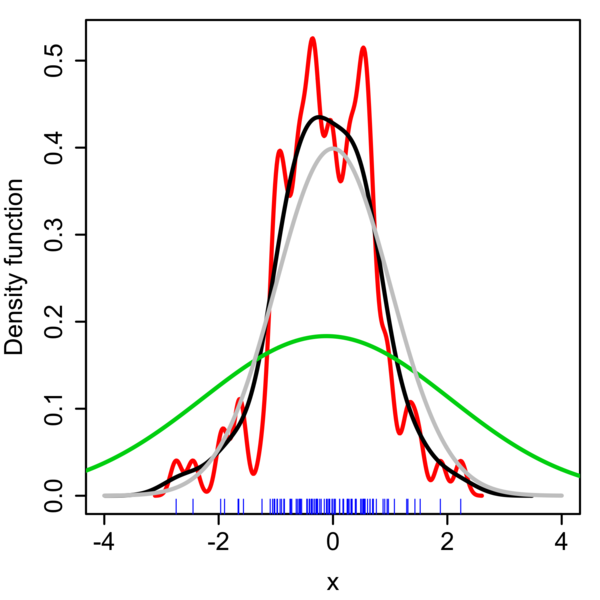
\includegraphics[width=0.5\textwidth]{bandwidth_selectors.png}
    \caption[Undersmoothing/Oversmoothing explanation]{The blue marks at the bottom of the plot shows a random sample from the Gaussian distribution. The grey curve shows the true density. The red curve visualises an undersmoothed estimation. The green curve visualises an oversmoothed estimation. The black curve is estimated using a near optimal bandwidth~\cite{wiki:kernel_density_estimation}.}
    \label{fig:bandwidth_selectors}
\end{figure}

\subsubsection{Finding a Good Bandwidth}
Finding the perfect bandwidth can be difficult. Which metrics define how good a given bandwidth is, depends on the domain of the data.

A simple approach is to eye-ball the results of using a variety of bandwidths. The result that gives the best looking bandwidth would then be chosen. This approach can give perfectly acceptable bandwidths, but the analyst has to have domain knowledge of the data. The results of this method are not reproducible, as different analysts will not deterministically choose their optimal bandwidths. Furthermore, it is also a tedious process~\cite{masteropgave}.

Another approach is to choose a bandwidth based on a metric of minimal errors. The idea is that an optimal solution will have the least errors. One method of doing this is to find the bandwidth with the lowest mean integrated squared error (MISE), as shown in \cref{eq:mise}.

\begin{equation}\label{eq:mise}
     E \int(\hat f_{h}(x) - f(x) )^2\mathrm{d}x
\end{equation}

In this method we take the integral of the squared difference between the estimate function $\hat f$ given bandwidth $h$ and the true density function $f$. We then multiply this with the expected mean value $E$ for the true density data. The intuition is that the bandwidth which will give the lowest area of error should be chosen. The hardest part of this method is to identify $f$~\cite{masteropgave}.

As noted in the introduction to this section, we will do a very simple bandwidth selection experiment. We therefore use a simpler metric of error called the sum of squared errors (SSE). The SSE is defined in \cref{eq:sse}.

\begin{equation}\label{eq:sse}
    \sum (\hat f_{h}(x) - f(x) )^2
\end{equation}

Here $\hat f_{h}(x)$ is the kernel density estimator $\hat f$ with bandwidth $h$ for a point $x$  and $f(x)$ is the actual density at point $x$. The idea of is to find the bandwidth that minimises the SSE.

The SSE formula defined in \cref{eq:sse} needs true density test data to be used as a benchmark for the performance of the bandwidth. In the perfect world, this test data should have the same structure as a real world crowd. We consider the problem of finding test data that matches a real world crowd as difficult, maybe even suitable for a project on its own. Instead, we will generate a simple pattern, that will illustrate how different bandwidths affect the kernel density estimation results.

We generate test data that takes the pattern of a chess board. This means that people has been placed such that the square alternates between two densities. The true densities are illustrated in \cref{fig:chessBoard-low1-high3-band5} where the blue squares have a density of 1 person per square metre and the turquoise squares have a density of 3 persons per square metre.

\definecolor{lowDensity}{HTML}{0967FD}
\definecolor{highDensity}{HTML}{00FFCF}

\begin{figure}[htbp]
\centering

\begin{tikzpicture}[x=1cm,scale=0.5]
    \foreach \x in {0,...,7} \foreach \y in {0,...,7}
    {
        \pgfmathparse{mod(\x+\y,2) ? "lowDensity" : "highDensity"}
        \edef\colour{\pgfmathresult}
        \path[fill=\colour] (\x,\y) rectangle ++ (1,1);
    }
    \draw (0,0)--(0,8)--(8,8)--(8,0)--cycle;
\end{tikzpicture}
    \caption[Chess board pattern]{Chess board pattern with blue squares having a density of 1 person per square meter and turquoise squares having a density of 3 person per square meter.}
    \label{fig:chessBoard-low1-high3-band5}
\end{figure}

The next section will give concrete data that shows how different bandwidths affect the density estimation.

\subsubsection{Effect of Bandwidth}

Using the chess board pattern introduced in the previous section, we will now get a better intuition of the choice of bandwidth. 

\begin{figure}[htbp]
\centering

\begin{subfigure}[c]{.32\linewidth}
    \centering
    
\includegraphics[width=\textwidth]{chessBoard-low1-high3-band1-density-subsquares.png}
    \caption{Bandwidth 1 metre}
    \label{fig:chessBoard-low1-high3-band1-cropped}
\end{subfigure}
%
\begin{subfigure}[c]{.32\linewidth}
    \centering
    
\includegraphics[width=\textwidth]{chessBoard-low1-high3-band5-density-subsquares.png}
    \caption{Bandwidth 5 metre}
    \label{fig:chessBoard-low1-high3-band5-cropped}
\end{subfigure}
%
\begin{subfigure}[c]{.32\linewidth}
    \centering
    
\includegraphics[width=\textwidth]{chessBoard-low1-high3-band10-density-subsquares.png}
    \caption{Bandwidth 10 metre}
    \label{fig:chessBoard-low1-high3-band10-cropped}
\end{subfigure}
%
\caption[Analysed chess board pattern with different bandwidths]{Cropped chess board pattern with blue squares having a density of 1 and turquoise squares having a density of 3. The bandwidth varies on the different subfigures.}
\label{fig:chessBoard-different-bandwidths}
\end{figure}

Let us look at how three different bandwidths change the kernel density estimation of the same data set. \Cref{fig:chessBoard-different-bandwidths} depicts three chess board patterns with varying bandwidths. \Cref{fig:chessBoard-low1-high3-band1-cropped} is very close to the structure of the chess board pattern, but there is some unwanted noise in the blue squares. We would say that the estimation is a little undersmoothed. \Cref{fig:chessBoard-low1-high3-band5-cropped} has a more blurry transition between each adjacent square, which means that the estimation is not really finding the hard transition of the underlying true data. There is however no noise inside each square. We would say that the estimation is a little oversmoothed. In \cref{fig:chessBoard-low1-high3-band10-cropped} we see a clear example of an oversmoothing bandwidth. Each square transition is still somewhat visible, but it is nowhere near the underlying true data.

Every bandwidth in \cref{fig:chessBoard-different-bandwidths} had some problems; Either the bandwidth was too low or too high. We will now try to determine a better bandwidth using the aforementioned SSE method. We iterate through a bandwidth interval from 1 metre to 5 metres with a step of 0.1 metre, because we know that the optimal bandwidth is around that interval. The result of the calculation is that the best bandwidth is 1.4 metre with an SSE of $5745.06$. \Cref{fig:chessBoard-low1-high3-band1.4-cropped} shows a crop of the chess board data with a bandwidth of 1.4 metre. We can see that this bandwidth indeed seems to be optimal; There is no noise inside the blue squares, and the square transitions are still following the underlying structure of the true density data.

\begin{figure}[htbp]
\centering

\includegraphics[width=0.32\textwidth]{chessBoard-low1-high3-band1-4-density-subsquares.png}
\caption[Analysed chess board pattern with bandwidth 1.4]{Cropped chess board pattern with blue squares having a density of 1 and turquoise squares having a density of 3. The bandwidth of 1.4 metres is calculated using a SSE method.}
\label{fig:chessBoard-low1-high3-band1.4-cropped}
\end{figure}

\subsubsection{Bandwidth Summary}

The above sample data is useful for giving an intuition of the effect of different bandwidths, but in order for the bandwidth selection to be useful in practice, one would have to do the bandwidth selection on data that represents the crowd to be analysed.


\kanote{summary af de teoretiske afsnit}

%% design and planning
\section{Analyser Design}\label{s3:analyser_design}

The analysis of the crowd factors of large events require a great amount of calculations. From the interviews with SmukFest we can expect numbers upwards of 50,000 people during peek hours, and there are many events dealing with much larger numbers of people, such as the Hajj \cite{website:Wikipedia-Hajj2}. If the application is to work on large scales, we need to consider the design of the analyser module, in order to keep the amount of calculations, network communication, and memory use to a minimum.

\subsection{Asynchronous Analysis}
\label{sub:Asynchronous_Analysis}

The first way we reduce the amount of calculations, is to do the analysis asynchronously from user requests. If we were to do a new analysis every time a user wants to see the crowd conditions for a given time period, multiple users requesting real-time analysis would quickly cripple the system. Instead we have a request-handler module, that handles the incoming requests and prepares them for the analyser. In order to fully benefit from this we also have to store completed analyses, such that identical requests can utilise the same results. This prompts the need for a storage module, which stores and catalogues completed analyses. This way the request-handler can bypass the analyser if the requested data is already available in storage, saving computation time.

This architecture allows us, and also require us, to have policies for the request-handler and storage modules. The policy for the request-handler should consider the priority of the incoming requests, whether it be first come first serve, or a priority based system where certain users are prioritised. Another possibility assuming that recently requested heatmaps are saved for some time is to rank requests based on the expected popularity, for instance the newer heatmap the more likely it is to be requested. The storage module also require a policy as to which data to keep and for how long to keep it. Once again different policies can be considered depending on the scope of the system. If we have enough space we can choose to keep all the analysed data, especially if we knew that the system would only run over a certain time period, for instance, the festival. If the system should be able to run indefinitely we would likely prefer to prioritise the data, and only keep a certain amount.

Given the asynchronous design, any data required by the analysis should be retrieved and prepared in advance, so that the analysis does not get unnecessarily delayed. This includes two parts, the first being the retrieval of position data from the aSTEP core, and the other being selection of the points which the analyser will analyse.

\subsection{Supplying Position Data}

Due to the nature of the velocity and heading-direction analysis, data preparation involves a short history of positions to be available. The direct approach of preparing data for each analysis and then deleting it once the analysis has been completed would likely cause an unnecessary amount of request to the aSTEP API. Take the example illustrated in \cref{memposexample} where an analysis is done for the time of $t_0$, where the last couple of positions for $t_{-1}$, $t_{-2}$, and $t_{-3}$ are also prepared. Then afterwards another analysis is done for time $t_{1}$, and we prepare data from $t_0$, $t_{-1}$, and $t_{-2}$. Here it would have been beneficial to retain $t_{-2}$, $t_{-1}$ and $t_{-0}$, since a lot of it overlaps with the analysis of $t_1$. Depending on the policy chosen for the request-handler, the data preparation should accommodate for future requests. Under the assumption that the most recent analysis would be the most requested or that we store all completed analyses indefinitely, it would be preferable to keep position data for the latest $n$ steps, where $t_{-n}$ is the oldest position used for finding the heading-direction and velocity. Different policies for the request handler will however affect the optimal choice of data kept in preparation.

\begin{figure}[htbp]
    \centering
    \begin{tabular}{rcccc}
        \nth{1} analysis: & $t_{-3}$ & $t_{-2}$ & $t_{-1}$ & $t_{0}$ \\
        \nth{2} analysis: & $t_{-2}$ & $t_{-1}$ & $t_{0}$  & $t_{1}$
    \end{tabular}
    \caption{Overlapping data required for analysis.}\label{memposexample}
\end{figure}


\subsection{Selection of Points to Analyse}
\label{s3:select_points}
Now that we have prepared the position data for the analyser, we have to select some points to analyse the local crowd factors for.

We divide the area to analyse into a grid of hexagons. In \cref{sub:kernelDensityEstimation} we assume that people are affected by the crowd factors in a radius away from them, resulting in a circular area of affection. The same assumption can also be used in the representation, meaning that the optimal representation would also display circles. The prblem meanwhile is that it is not possible to make a perfect circular tessellation on a square plane. Meanwhile hexagons have the nice property that a regular tiling can be made with them, i.e. they can be placed in a pattern where they cover an entire area without overlapping nor leaving gaps. While squares also hold this property, we prefer hexagons since they are the closest resembling regular tiling of  a circle with radius of the bandwidth. \Cref{fig:analysis_hexagon_divide} provides an illustration of this. The centre of each hexagon is a point that the analyser should analyse.

\begin{figure}[htbp]
\centering
\begin{tikzpicture} [
    hexa/.style= {shape=regular polygon,
                  regular polygon sides=6,
                  minimum size=1cm, draw,
                  inner sep=0,anchor=south,
                  fill=lightgray}
    ]

\foreach \j in {0,...,4}{% 
     \ifodd\j 
         \foreach \i in {0,...,3}{\node[hexa] (h\j;\i) at ({\j/2+\j/4},{(\i+1/2)*sin(60)}) {.};}        
    \else
         \foreach \i in {0,...,3}{\node[hexa] (h\j;\i) at ({\j/2+\j/4},{\i*sin(60)}) {.};}
    \fi}
\end{tikzpicture}
\caption{Illustration of dividing the area to analyse into a grid of hexagons.}\label{fig:analysis_hexagon_divide}
\end{figure}


\subsection{Lightweight Results}

While we are primarily concerned with reduction of complexity and computation time of the analysis, there are other aspects of the design that require some attention. The amount of data required for a single analysis can reach rather large sizes, and in order to keep network traffic with potentially multiple users to a minimum, the analyser should, as a bi-product of its analysis, reduce the size of a completed analysis. In other words, a lightweight data structure for the results should be conceived. 

The conceived data structure stores the result of the crowd condition analysis along with the matching position, by taking advantage of the uniform distribution of analysed points in a grid. This allows the data structure to only keep track of the global position of a single point and then the distance between points, as well as the dimensions of the analysed area. From this information a client can recreate the grid and start plotting the sequential data accordingly.

This removes the need to send a global position for each point, however it does require the structure to hold every single point in the grid, even if the point is not affected by any person and all its values are zero.


\subsection{Summary}

This asynchronous design of the analyser allows us to divide the analysis into separate parts, which in turn allow for assembly line approach where as much preparation as possible can be done ahead of time. The analyser can run continuously, without being slowed down by communication with data sources. The different parts needs to be implemented with policies which govern their behavior. The design suggests an implementation where policies can be substituted, in order to easily tailor the system to different uses.


%% implementation
\section{Implementation}

In this section we will cover the important parts of the implementation that was done during this sprint. First we will discuss the implementation of the analyser, and the efforts made towards a faster analysis. We will also briefly cover the implementation of the client side visualisation.

\subsection{Implementation of the Analyser}\label{s3:analyser_implementation}

In order to fully understand the need for a good implementation of the analyser, we start with a quick run-down of the complexity of the unoptimised algorithm implemented directly as derived in \cref{subsec:estimatingCrowdFactors}. The pseudo code implementation can be seen in \cref{alg:unoptimised_algorithm}.

\begin{center}
\captionof{algorithm}{Unoptimised algorithm}\label{alg:unoptimised_algorithm}
\begin{algorithmic}[1]

\Function{Analyser}{List points, List people, Bandwidth h}
\State Densities $\gets$ empty List
\State Velocities $\gets$ empty List
\State Turbulence $\gets$ empty List
\State Pressure $\gets$ empty List
\ForAll{points, x}
    \State KernelSum $\gets 0$
    \ForAll{people, P}
        \State KernelSum $\gets$ KernelSum $+$ \Call{Kernel}{|x - P|}
    \EndFor
    \State \Call{Densities.Add}{KernelSum $\cdot\; 2 / (\pi \cdot h^2)$}
\EndFor

\ForAll{points, x}
    \State KernelSum $\gets 0$
    \State VelocitySum $\gets 0$
    \ForAll{people, P}
        \State VelocitySum $\gets$ VelocitySum $+$ \Call{VelocityOf}{P} $\cdot$ \Call{Kernel}{|x - P|}
        \State KernelSum $\gets$ KernelSum $+$ \Call{Kernel}{|x - P|}
    \EndFor
    \State \Call{Velocities.Add}{VelocitySum $/$ KernelSum}
\EndFor

\ForAll{points, x}
    \State KernelSum $\gets 0$
    \State TurbuSum $\gets 0$
    \ForAll{People, P}%
        \State TurbuSum $\gets$ TurbuSum $+$ \Call{DirectionOf}{P} $\cdot$ \Call{Kernel}{|x - P|}
        \State KernelSum $\gets$ KernelSum $+$ \Call{Kernel}{|x - P|}
    \EndFor
    \State \Call{Turbulence.Add}{TurbuSum $/$ KernelSum}
\EndFor

\ForAll{points, x}
    \State KernelSum $\gets 0$
    \State PressSum $\gets 0$
    \ForAll{People, P}
        \State VelocityDiff $\gets$ |\Call{VelocityOf}{P} $-$ x.LocalVelocity|
        \State PressSum $\gets$ PressSum $+$ (VelocityDiff)$^2$ $\cdot$ \Call{Kernel}{|x - P|}
        \State KernelSum $\gets$ KernelSum $+$ \Call{Kernel}{|x - P|}
    \EndFor
    \State \Call{Pressure.Add}{x.LocalDensity $\cdot$ (PressSum $/$ KernelSum)}
\EndFor
\State\textbf{Return} (points, Densities, Velocities, Turbulence, Pressure)
\EndFunction
\end{algorithmic}
\end{center}

This algorithm has an asymptotic time complexity of $$\mathcal{O}(\text{points} \cdot \text{people})$$ which at first might seem decent. However, recall that the amount of points is related to the resolution, meaning that a point for every square meter at SmukFest, will result in 230,000 points~\cite{smukFacts}. Combining this with potentially 50,000 festival guests~\cite{smukFacts}, we reach an amount of potential calculation, for each analysis, that a regular server will struggle to evaluate within the real-time requirement of \cref{sec:s3_requirements}. We therefore want to reduce the complexity as much as possible.


\subsubsection{Reducing Complexity}

The first thing we need to reduce is the complexity. This would mean reducing either of the terms of the complexity, namely points or people.

All points have to be considered since these are the points we want to find the local crowd factors for. We could reduce the amount of points we want to analyse on, but this would not reduce the complexity of the analyser itself. If we want to reduce the complexity we need to reduce the amount of people iterated through per point. Considering that the kernel function will return zero for any person further away from the point than the bandwidth, we can reduce the complexity given that a reasonable bandwidth is used. This also relies on the reasonable assumption that people take up space, and that therefore we can only have a certain amount people inside a given bandwidth.

Before we can utilise the drop off point of the kernel function, we need a way to check if a person is further away than the bandwidth, without having to iterate through all the people. This can be done using R-trees. An R-tree is a data structure that takes $\mathcal{O}(n)$ to build, and allows us to do range searches in $\mathcal{O}(log(n))$ \cite{rtree}. If we start the analysis with building an r-tree of the people, finding the people withing the bandwidth for each point would only take $\mathcal{O}(log(n))$ time to find, where n is the amount of people. The amount of people found using the range trees is here denoted with the function \emph{PeopleWithinBandwidth}. This would give us the complexity of $$\mathcal{O}(\text{people} + \text{points} \cdot log(\text{people}) \cdot \text{PeopleWithinBandwidth(h)})$$

Considering that there is a physical limit as too how dense people can be packed, the function \emph{PeopleWithinBandwidth(h)} would in the worst case return $h^2 \cdot \pi \cdot \text{maxDensity}$. Since we at runtime will have a constant bandwidth, $h$, and the max density is also constant, \emph{PeopleWithinBandwidth(h)} will have a constant worst case. The final complexity is therefore $$\mathcal{O}(\text{points} \cdot log(\text{people}))$$

\subsubsection{Parallel Computation}

Another way to decrease the time spent on the analysis, is to take advantage of the embarrassingly parallel problem of calculating a kernel value for each point. Since none of the calculations done for any individual point affect the the other points, we can calculate their values in parallel, meaning that we in principle can have an individual thread for each point.

\subsubsection{An Optimised Algorithm}
All these considerations leads us to the pseudo-code for the optimised analyser algorithm. The algorithm is split into two functions and can be seen in \cref{alg:revised_algorithm}. The first function on \cref{firstfunc} is the analyser function. This is basically a for-loop with two objectives: Find the relevant people for each point through an R-tree, and call the \emph{analysePoint} function. This for-loop represents the embarrassingly parallel part of the problem. It should be noted that while the same R-tree is used for multiple points, only read actions are done, and as such there are no race conditions.

The second function on \cref{secondfunc} of the algorithm, is the part where the local crowd factors are calculated. The primary change here, is the reduction of four for-loops, down to two. The primary reason for this reduction is the repeated calls to the \emph{Kernel} function, which calculates a given person's kernel value. Since this is a rather costly calculation, we store the result of the calculation on \cref{tmpkernel}, and use this value for each factor. Note that on \cref{secondkernel}, another call is made to the \emph{Kernel} function. In the actual implementation this is avoided through a technical workaround in the first for-loop. However we have omitted that detail in order to keep the pseudo-code less complicated.

On line \cref{firstval} through \ref{lastval} we introduce summation variables, which will store the non-normalised values. Note that the value for velocity on \cref{veloval} is a vector. We then reach the first for-loop, which will iterate through every person in the reduced list, and add that person's crowd factors to the respective accumulator after it has been adjusted by the kernel value.

At \cref{validhead} we have an \emph{if} statement, which makes sure that the heading direction is not invalid, in accordance with the solution presented in \cref{subsub:turbu}, to the problem of still standing people. If the heading direction is valid, the accumulator is updated on \cref{adjustturbu} and \ref{turbusum}, along with the separate kernel value summation on \cref{turbukernel}.

On \cref{nullcheck} we have an \emph{if} statement, which checks if the point has a kernel value of $0$, which would cause a division error in \cref{secondres,lastpres}. The same principle goes for the \emph{if} on \cref{turbunullcheck} and the division on \cref{thirdres}.
Then at \cref{firstres} through \ref{thirdres} the first three factors are normalised, and on \cref{firstpres} through \ref{lastpres} we calculate the local crowd pressure. We finally return the result on \cref{return}.

This algorithm holds the desired complexity of $$\mathcal{O}(\text{points} \cdot log(\text{people}))$$

assuming the previously found constant maximum of people within an area.

\begin{center}
\captionof{algorithm}{Optimised algorithm using RTree range search}\label{alg:revised_algorithm}
\begin{algorithmic}[1]
\Function{Analyser}{List points, rTree t, Bandwidth h}\label{firstfunc}
\State Result $\gets$ Empty List 
\ForAll{points, p}
    \State CulledPeople $\gets$ \Call{t.inRange}{h,p} 
    \State Result $\gets$ Result + \Call{analysePoint}{p,CulledPeople}
\EndFor
\State \textbf{Return} Result

\EndFunction

\Function{analysePoint}{Point x, List people}\label{secondfunc}


\State KernelValSum $\gets 0$\label{firstval}
\State NonNormVeloSum $\gets vector(0.0,0.0)$\label{veloval}
\State NonNormTurbuSum $\gets 0$
\State TurbuKernelValSum $\gets 0$\label{lastval}


\ForAll{People, P}
    \State TmpKernelVal $\gets$ \Call{Kernel}{|x - P|}\label{tmpkernel}
    \State KernelValSum $\gets$ KernelValSum + TmpKernelVal
    \State NonNormVeloSum $\gets$ NonNormVeloSum + P.Velocity * TmpKernelVal
    \If{P.HeadingDirection is valid}\label{validhead}
        \State AdjustedTurbu $\gets$ P.HeadingDirection $\cdot$ TmpKernelVal\label{adjustturbu}
        \State NonNormTurbuSum $\gets$ NonNormTurbuSum $+$ Adjusted Turbu \label{turbusum}
        \State TurbuKernelValSum $\gets$ TurbuKernelValSum + TmpKernelVal\label{turbukernel}
    \EndIf
\EndFor

\If{KernelValSum is 0}\label{nullcheck}
    \State \textbf{Return} (0,(0,0),0,0)
\Else
    \State Density $\gets$ KernelValSum $\cdot \; 2 / (\pi \cdot h^2)$\label{firstres}
    \State Velocity $\gets$ NonNormVelocitySum / KernelValSum \label{secondres}
    \State Turbulence $\gets$ 0
    \If{TurbuKernelValSum is 0} \label{turbunullcheck}
        \State Turbulence $\gets$ 1 - ( NonNormTurbuSum / TurbuKernelValSum )\label{thirdres}
    \EndIf
    \State VelocityDiffSum $\gets$ 0 \label{firstpres}
    \ForAll{People, P}
        \State VelocityDiff $\gets$ |P.velocity - Velocity|$^2 \cdot$ \Call{Kernel}{|x - P|}\label{secondkernel}
        \State VelocityDiffSum $\gets$ VelocityDiffSum $+$ VelocityDiff
    \EndFor
    \State Pressure $\gets$ Density $\cdot$ ( VelocityDiffSum / KernelValSum )\label{lastpres}
\State \textbf{Return} (x, Density, Velocity, Turbulence, Pressure)\label{return}
\EndIf
\EndFunction
\end{algorithmic}
\end{center}
\subsection{Customized Visualisation}\label{sec:own_leaflet_plugin}

Up till this point we have used multiple different Leaflet plug-in libraries for visualisation. These libraries were however not adequately flexible for the data we have to visualise. We therefore created our own Leaflet plug-in, giving us the ability to tailoring the visualisations to our needs.

Every Leaflet plug-in library we explored has its own assumptions on how data should be visualised, and none of those assumption satisfied our needs. For example, all libraries use a global scaling of densities, meaning the density visualisation of a point depends on the density of other points. Additionally, we had no control over the shapes used in the visualisations.

Because of this, we decided to create our own Leaflet plug-in based on Leaflet.heat. The goal of this plug-in is to allow us to experiment with different visualisation techniques more freely. By creating our own plug-in, we have complete control of how the data is drawn on the map. This means that we can render the visualisations in a very specific fashion that suits our needs.